\section{Il problema}

\begin{frame}
	\sectionpage
	\centering
\end{frame}

\begin{frame}
	\frametitle{Reti complesse}
	\centering
\end{frame}

\begin{frame}
	\frametitle{Sei gradi di separazione}
	\textit{"Ho letto che ognuno di noi su questo pianeta è separato dagli altri solo da sei persone. 
		Sei gradi di separazione tra noi e tutti gli altri su questo pianeta [...]\\ una tortura cinese essere così vicini ma dover trovare sei persone giuste per il collegamento."}
	\begin{flushright}
		\textit{Ouisa Kittredge}\\
		\textit{Six Degrees of Separation}
	\end{flushright}

	% \pause
	
	\begin{figure}[h]
		\centering
		\begin{minipage}[t]{.49\textwidth}
			\centering
			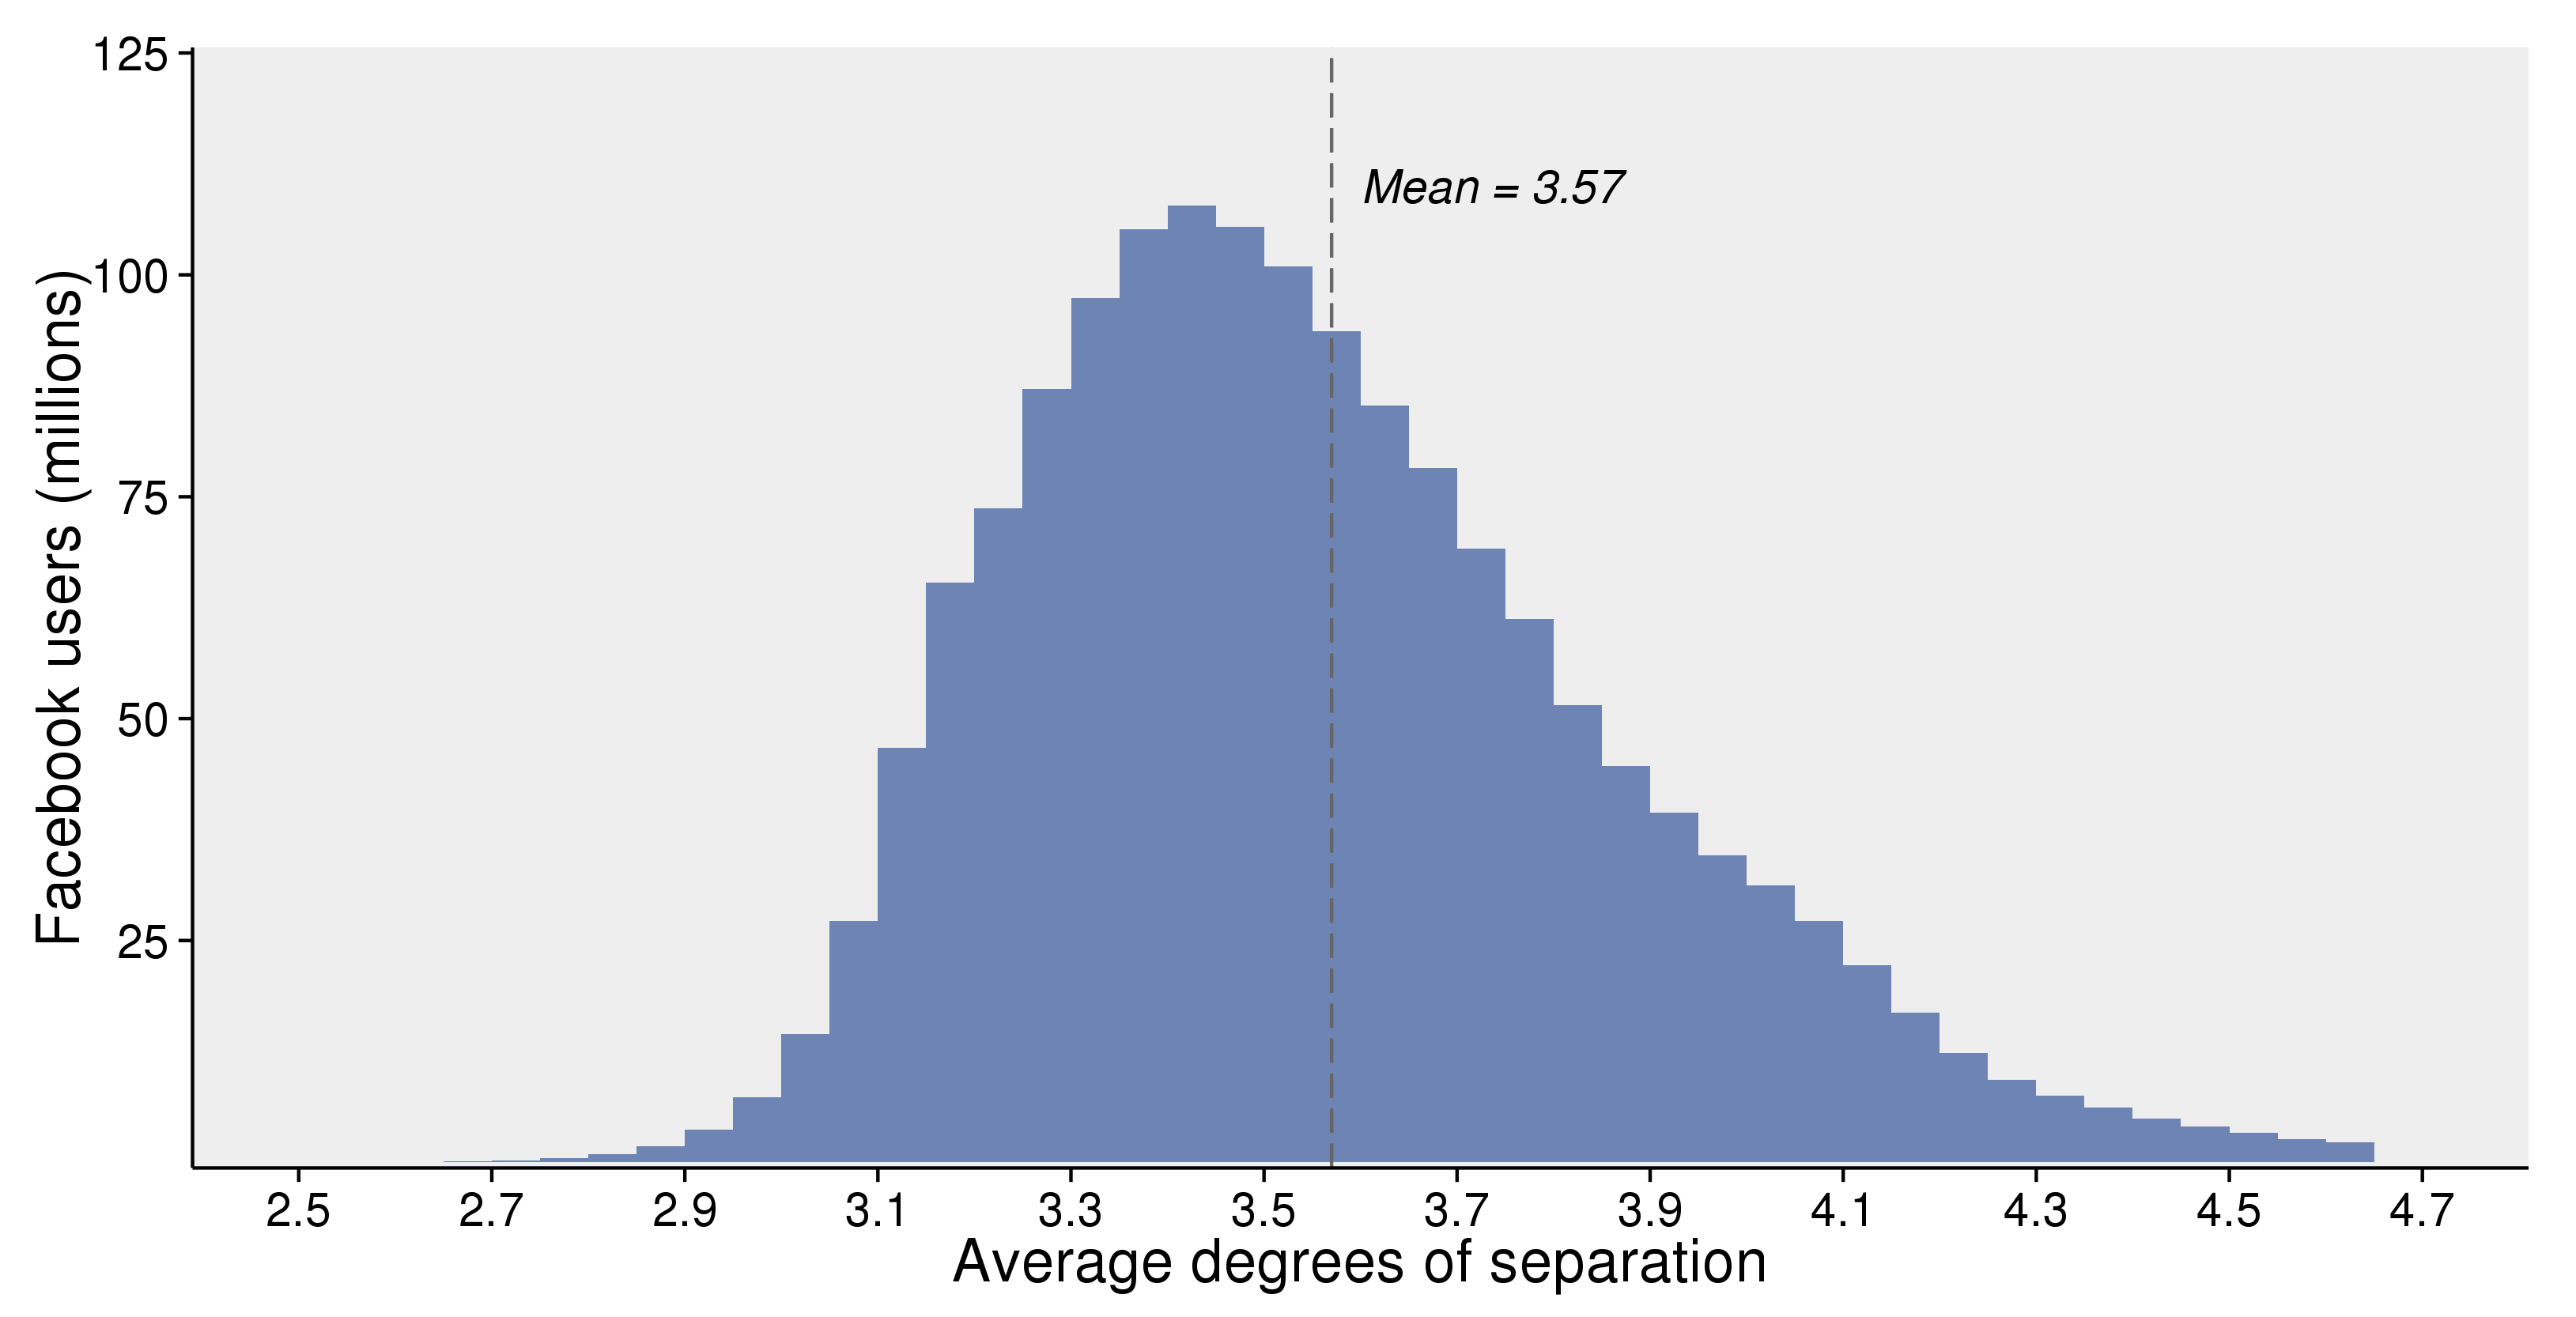
\includegraphics[width=0.9\textwidth]{images/facebook}
			\caption{In facebook la separazione media tra gli 1.6 miliardi di utenti registrati è $3.57$.\\ \textit{Fonte: facebook research, Feb 2016}}
		\end{minipage}\hfill
		%\pause
		\begin{minipage}[t]{.49\textwidth}
			\centering
			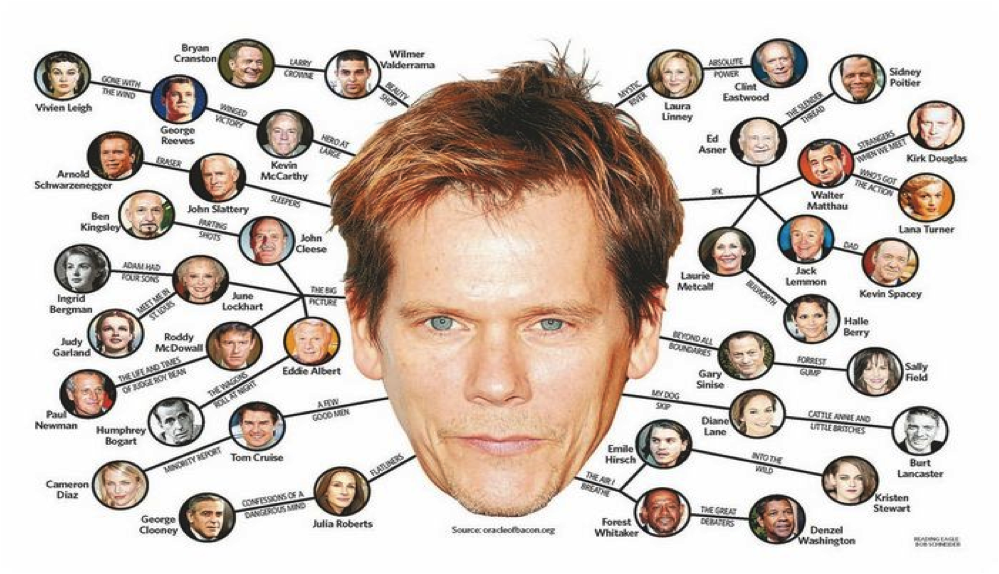
\includegraphics[width=0.9\textwidth]{images/2_kevin_bacon}
			\caption{La distanza media di collaborazioni dall'attore Kevin Bacon è $3$, il $98\%$ degli attori è a distanza minore uguale a $6$.\\ \textit{Fonte: IMDb, Ott 2017}}
		\end{minipage}
	\end{figure}
	
\end{frame}

\begin{frame}
	\frametitle{Reti etichettate e $q$-grammi}
	\centering
\end{frame}

\begin{frame}
	\frametitle{Indici di similarità}
	\centering
\end{frame}

\begin{frame}
	\frametitle{Il problema}
	\centering
\end{frame}

\begin{frame}
	\frametitle{Applicazioni pratiche}
	\centering
\end{frame}
